\section{Introduction}

The biggest problem of artificial intelligence is that we don't know what natural intelligence is. Unfortunately there are no aliens so far who would be able to demonstrate non-human intelligence, and examples on Earth lack certain substance. Rosalind Picard in her article indicated: "There may exist a kind of alien intelligent living system, something we’ve never encountered, which achieves its  intelligence without having anything like emotion. Although humans are the most marvellous example of intelligence we have, and we wish to build systems that are natural for humans to understand, these reasons for building human-like systems should not limit us to thinking only of human abilities." \cite{affectivecomputingchallanges}

There are several domains that still remain unclear: creativity, intuition, insight and consciousness that prevent us from answering the question: "How David Lynch could create Mulholland Drive or Picasso could create Guernica?". One aspect of modern AI is affective computation that become more and more important it is based on several domains: psychology: \cite{natureofemotions, appraisal_determinants_of_emotions, appraisal_considered_as_a_process, putting_appraisal_in_context, sex_differencies}, neuroscience: \cite{emotionsbraintorobot, parsingreward, neuromodulatory, cubeofemotions, natureofemotions, putting_appraisal_in_context, anatomic}, computer science: \cite{intelligent_machinery, emotionandsociable, senticcomputing, hourglass, affectivemodelofinterplay, affectivecomputing, dont_worry_be_happy, hourglass, senticcomputing, parsingreward, emotionsbraintorobot, motivationalrewardframework, roleofemotions, computationalmodelsemotionscognition}. Although there are still only several computational emotions models created \cite{computationalmodelsemotion, computationalmodelsemotionscognition, evaluatingcomutationalmodel, threelevel}.

Turing stated in his report ``Intelligent Machinery'' \cite{intelligent_machinery} that idea of intelligent machines "cannot be wholly ignored, because the idea of 'intelligence' is itself emotional rather than mathematical".
There is an interconnection between emotions and rational thought. Marvin Minsky in his book "The emotion machine" proposed that emotions are inseparable from thinking: "Emotional thinking: A flash of impatience or anger can cut through what seems like a hopelessly tangled knot. Each such 'emotional way to think' is a different way to deal with things, and some can increase your persistence or courage, while others can help you simplify things. In any case, after each such change, you may still want to pursue some similar goals, but now you'll see them from new points of view — because each switch to a new Way to Think may initiate a large-scale cascade. Then, depending on how long those changes persist, you (or your friends) might recognize this as a change in your emotional state".

This article is dedicated to model of affective computation based on neuroscientific monoamine model of neuromodulation and affects in human brain and derivative possible influence of emotions(affects) \footnote{In this article we use affects and emotions as notions with the same or close meaning, usually affects is used in sections dedicated to affects theory \cite{tomkins1, tomkins2, tomkins3} or derivatives \cite{cubeofemotions}, emotions on the other hand is used in context of Plutchik ``wheel of emotions'' context \cite{natureofemotions}.} on computational processes in Marvin Minsky's cognitive architecture \cite{emotionmachine}. It could be considered as a base of affective computation framework and we hope could be used in several domains like:

\begin{enumerate}
 \item  Advertisement
 \item  Emotional behavior simulations
 \item  Robotics
 \item  Intellectual assistants
 \item  Estimating human behaviour
 \item  Nursing software and robotics
\end{enumerate}

\section{Bases}

Starting from the top we first reviewed several psychological models of emotions. Then we tried to understand the low level nature of emotions that brought us to neurochemical base of emotions. As we got the picture of human emotional processes we mapped them to cognitive architecture to gain AI basis. This approach is represented on the figure~\ref{3_bases}.

\begin{figure}
\begin{center}
 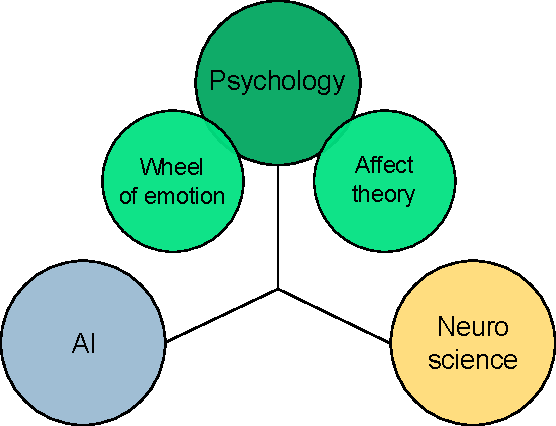
\includegraphics[height=3.5cm]{figure1_3_bases}
\end{center}
\caption{Theoretical bases of current work.}
\label{3_bases}
\end{figure}

Firstly we wanted to gain overall picture of human emotional processes. It could be understood as combination of high level processes and model that triggers processes steps. This lead us to the first base: the evolutionary psychology theory of Plutchik "Wheel of emotions" \cite{natureofemotions}. In comparison to other classifications of emotions it provides complete picture of basic and combination of basics into high level taking in account emotional processes (feedback loops). For extensive description see Emotional Feedback Loops section. We adapted feedback loops into Model of six \cite{emotionmachine} thinking levels of Marvin Minsky's cognitive architecture.

As we gained overall picture of th human emotions, we faced the problem of low level mechanism that actually triggers the affects (emotional states), this leads us to neurobiological hypothesis of L\"{o}vheim: neuromodulatory base of emotions \cite{cubeofemotions}. ``Cube of emotions'' by it self based on the theory of affects by Tomkins \cite{primer_affect_psychology, tomkins1, tomkins2, tomkins3}. We used Tomkins theory of affects as the base for low level(basic) emotions and appraisal \cite{primer_affect_psychology, appraisal_considered_as_a_process, appraisal_determinants_of_emotions, putting_appraisal_in_context}.

We gained proper philosophical context by means of Marvin Minsky book ``The emotion machine''. This book shades the light on really complex phenomena like: consciousness, thinking, levels of mental activities and so on. We mapped all the theories described above on Marvin Minsky's cognitive architecture described in his book "The emotion machine" \cite{emotionmachine}.

\section{Emotional Feedback Loops}

Robert Plutchik created the three dimensional model \cite{natureofemotions} called "Wheel of emotions", that we used to describe subjective perception of emotions. There are eight basic emotions grouped in pairs:

\begin{enumerate}
 \item  Joy - sorrow
 \item  Anger - fear
 \item  Acceptance - disgust
 \item  Surprise - expectancy
\end{enumerate}

Model presented above could be understood as the base for the subjective picture of emotions. The other indeed important for understanding the emotions aspect presented by Robert Plutchik is emotional processes or feedback loops. He introduced 8 steps processes:

\begin{enumerate}
 \item{stimulus event}
 \item{inferred cognition}
 \item{feeling state}
 \item{physiological arousal}
 \item{impulses to action}
 \item{overt behaviour}
 \item{effect}
\end{enumerate}

Robert Plutchik describes it as: ``Overall, emotion is a kind of homeostatic process in which behavior mediates progress toward equilibrium; I call it a behavioral homeostatic, negativefeedback system. Emotion is a chain of events made up of feedback loops. Feelings and behavior can affect cognition, just as cognition can influence feeling.'' \cite{natureofemotions}. Actions feeling state and physiological arousal are done in parallel. This is overall hight level template of all emotional processes of animals and humans. We interpreted this processes in four layers of Marvin Minsky's ``Model of six'' our interpretation is not direct we combined inferred cognition with feeling state and physiological arousal in affective appraisal and neuromodulation, we selected cognitive appraisal as separate step and put it on learned reactions layer. The distinction between affective appraisal and cognitive appraisal was inspired by \cite{emotionsbraintorobot} the potential neuromodulation pathway: from spinal cord, to hypothalamus and nucleus of the solitary tract then to amygdala and septum and then to cingulate cortex and frontal cortex, so firstly every stimulus is been responded by low level: spinal cord, to hypothalamus and nucleus of the solitary tract then to amygdala and septum, non-consciously, and then cingulate cortex and frontal cortex could impact to the whole processing consciously in case of frontal cortex. 
Mapping of emotional feedback loops to ``Model of six'' is presented on the figure~\ref{orchestra_of_emotions}.

\begin{figure}
%\vspace{10cm}
\begin{center}
 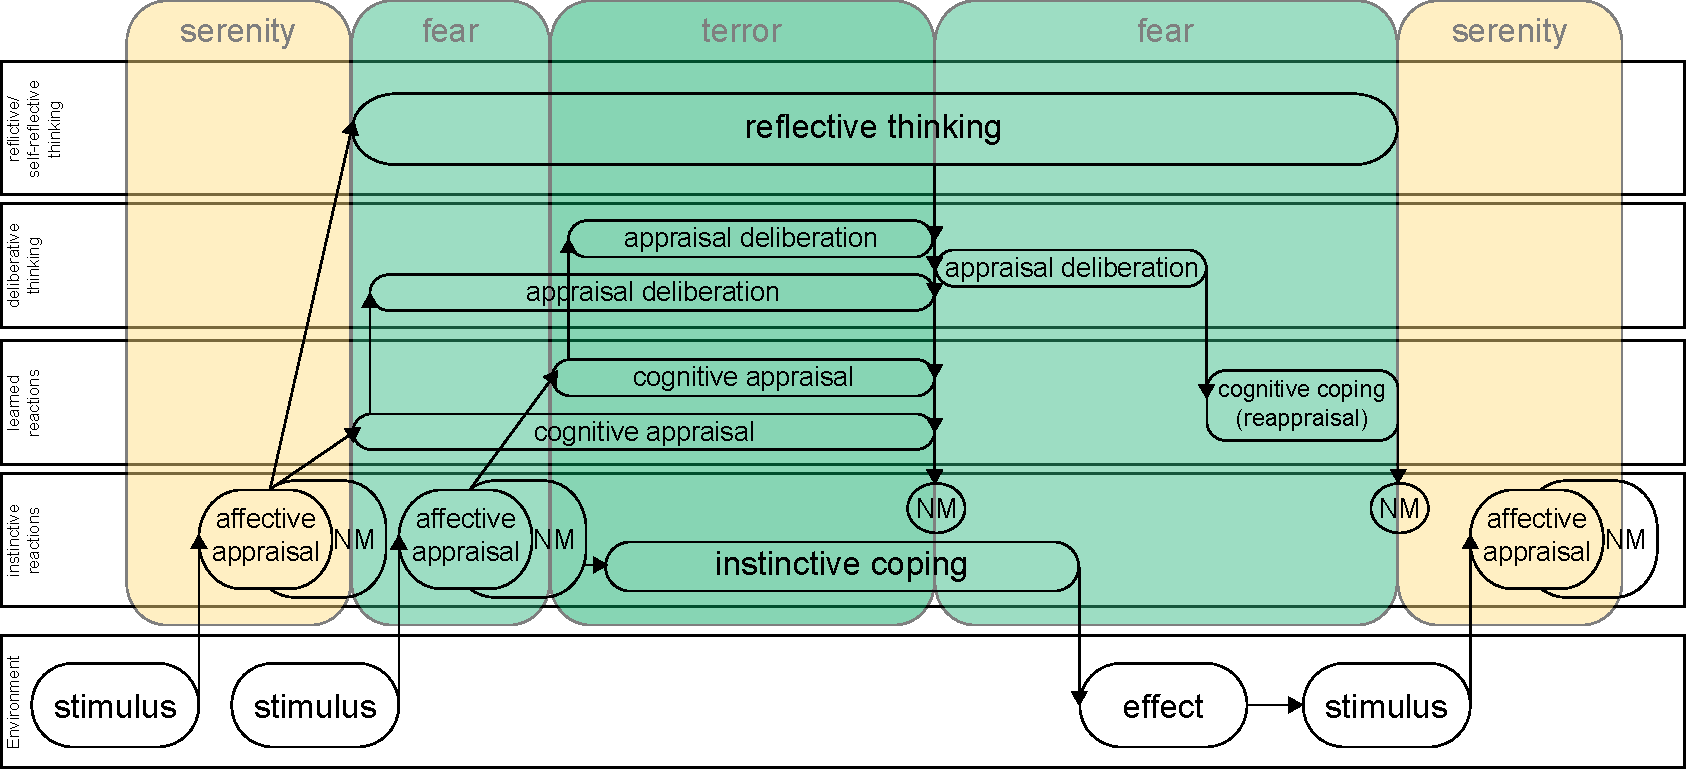
\includegraphics[height=10cm, angle=90]{figure2_orchestra_of_emotions}
\end{center}
\caption{Orchestra of emotions \label{orchestra_of_emotions}}
\end{figure}

We use four of the six layers just for the purpose of this example. Self-conscious reflections layer could influence emotions; for example evaluation of self as not progressing could cause sorrow or even depression, but it was not shown on the diagram.

We correspond instinctive reactions layer with non-conscious, innate, affective responses that mainly takes palace in: hypothalamus and amygdala, only after the frontal cortex is triggered in stimulus processing becomes conscious. This way any stimulus is being processed first unconsciously; this is shown as affective appraisal oval, and then consciously, this is shown as cognitive appraisal oval.

Using a concrete example presented on figure~\ref{orchestra_of_emotions}: first stimulus triggers affective appraisal and affective appraisal triggers neuromodulation. Neuromodulation triggers an emotional state switch from serenity to fear, depicted by yellow and green rectangle. Emotional states are represented as rounded rectangles on the diagram. Affective appraisal triggers cognitive appraisal and reflective thinking. Actions like appraisals, deliberations, copings and neuromodulations are represented as ovals on the diagram, initiation or triggering are shown on diagram as arrows. Cognitive appraisal in its turn initiates a appraisal deliberation process. Meanwhile second stimulus triggers second affective appraisal and its neuromodulation switches emotional state from fear to terror. Second affective appraisal triggers cognitive appraisal that in its turn initiates second appraisal deliberation. Then reflective thinking process estimating all activities in mind realizes that it's too emotional now and then stop all appraisal related processes and starts new coping oriented deliberation and switches emotional state via neuromodulation from terror to fear. Third appraisal deliberation selects cognitive reappraisal as coping strategy and this coping strategy is executed and switches emotional state back to serenity (via neuromodulation).
In parallel to all cognitive and reflective process the second affective appraisal initiates non-conscious instinctive coping strategy and it when applied created an effect over environment and this effect is been appraised again as stimulus.

\section{Neuromodulatory Basis of Artificial Emotions}

... Add citations, Oversimplified.

Hugo L\"{o}vheim in 2012 published his article "A new three-dimensional model for emotions and monoamine neurotransmitters" \cite{cubeofemotions}. He described three dimensional model of emotions. Axes of the model are neuromodulators (monoamines): serotonin, dopamine, noradrenaline. ``As each of these three monoamine systems probably represents a different aspect of emotion, a hypothetical three-dimensional space for possible combinations is formed. It is evolutionarily rational that the monoamine systems are mutually orthogonal as this maximizes the amount of information that can be transmitted, however, although likely, this needs to be further established empirically. It is important to note that as long as none of the monoamines transmit exactly the same information as any other (which seems unlikely), there will still be a three-dimensional space. For simplicity, in this article the monoamines axes have been depicted as mutually orthogonal.
... 
That each monoamine neurotransmitter represents a different aspect of emotion should not, however, be interpreted to mean that the monoamines are independent. There are probably complex systems of feedback and reciprocal control where the monoamine systems interact and affect each other. These interactions probably contribute to the dynamics of the monoamine systems. It is also noteworthy that the total ‘‘out-effect’’ in a monoamine axis is a function of the amount of signal substance that is released into the synaptic cleft, the rate of reuptake and degradation of the transmitter substance as well as the type, number, sensitivity and specificity of post-synaptic receptors. Complex feedback mechanisms regulate these factors.''


Vertexes are affects from Tomkins affect theory \cite{primer_affect_psychology}. ``The psychologist Silvan Tomkins devoted his life to the study of emotions and developed an elaborate and comprehensive theory of basic emotions[85–87,89]. Tomkins identified eight basic emotions, which he labeled with one word for the emotion when it was of low intensity and another word for the same emotion at a higher intensity[98,99]. Tomkins referred to basic emotions as ‘‘innate affects’’ where affect, in his theory, stands for the ‘‘strictly biological portion of emotion’’[83]. According to his theory, these are the eight basic emotions:''

\begin{enumerate}
 \item  Enjoyment/Joy
 \item  Interest/Excitement
 \item  Surprise
 \item  Anger/Rage
 \item  Disgust
 \item  Distress/Anguish
 \item  Fear/Terror
 \item  Shame/Humiliation
\end{enumerate}

Hugo L\"{o}vheim gives extended explanation of mapping of each neurotransmitter to group of emotions:


\subsection{Fear/terror and anger/range}

``Both of the basic emotions, fear/terror and anger/rage, are supposedly high-dopaminergic and therefore coupled to reinforcement[9,101–104]. This seems logical when one considers the great evolutionary value of learning about those dangerous situations in which these negative basic emotions are triggered. It has been found that laboratory rats easily learn to avoid various stimuli presented simultaneously as something innately scary (such as a cat)[34]. The rewarding effect of these basic emotions might also possibly explain why certain people continue to seek so-called adrenaline rushes. ... Both fear/terror and anger/rage are here further assumed to be low-serotonergic, as these emotions are triggered when the individual feels threatened or under pressure, and therefore probably has an inner feeling of weakness. Aggression has also been coupled to serotonergic deficit in many studies, supporting the placement of anger/rage on the low-serotonergic side[10,19,27,28,52,53].''



From our perspective this is the base of objective non-conscious emotional brain reaction to stimulus. On the other hand according to ``Emotions: from brain to robot'' \cite{emotionsbraintorobot} there are four following neuronal systems involved in emotional processing:

\begin{enumerate}
 \item Hypothalamus
 \item Amygdala
 \item Frontal cortex, 
 \item Cingulate cortex
\end{enumerate}

We roughly correspond non-conscious instinctive reactions layer of "model of six" \cite{emotionmachine} with hypothalamus and amygdala, while conscious processes and learned reactions, deliberative thinking, reflective thinking, self-reflective thinking, self-conscious reflections with frontal and cingulate cortex. This approach could be understood as subjective emotions to objective brain reaction mapping. This is fundamental for representation of emotional processes on computational system parameters.

\section{Neuromodulators to Computing Parameters Mapping}

... Expand.

Our understanding of the role of neuromodulators \cite{cubeofemotions, emotionsbraintorobot} is represented in following mapping of neuromodulators to computing system parameters, the figure~\ref{cube_of_parameters}.

\begin{figure}
%\vspace{5cm}
\begin{center}
 \includegraphics[height=7cm]{figure3_cube_of_parameters}
\end{center}
\caption{Cube of parameters}
\label{cube_of_parameters}
\end{figure}

\begin{enumerate}
 \item  Generic:
 \begin{enumerate}
  \item  Computing power: noradrenaline
  \item  Memory distribution (attention): noradrenaline
  \item  Learning: serotonin, dopamine
  \item  Storage: serotonin, dopamine
 \end{enumerate}
 \item  Decision making/reward processing:
 \begin{enumerate}
  \item  Confidence: serotonin
  \item  Satisfaction: serotonin
  \item  Motivation, wanting: dopamine
  \item  Risky choices inclination: noradrenaline
  \item  Number of options to process: noradrenaline
 \end{enumerate}
\end{enumerate}

\subsection{Generic}

\emph{Computing power}: distribution and priority of parallel process or load balancing, is impacted by noradrenaline: the higher the level of noradrenaline is the more computing power must be concentrated on current activity (neuromodulator regulating attention).

\emph{Working memory(short term)} distribution and concentration is impacted by noradrenaline (attention).

\emph{Learning} is impacted by serotonin and dopamine: dopamine plays major role in activation of previously remembered patterns and serotonin in pattern generation.

\emph{Storage} management (long term memory) is impacted by both by serotonin and dopamine, higher concentrations of both neuromodulators makes system better remember stimulus. In general, strong emotions generate more persistent memories.

\subsection{Decision making}

This decision making is done mainly in deliberation and learned reaction layers of model of six.
Parameters: confidence, satisfaction, risky are used to highlight actions stored(remembered).

\emph{Confidence and satisfaction} of the system is directly influenced by serotonin.

System is more \emph{motivated} under the influence of dopamine.

System tends to choose \emph{risky} actions under the influence of noradrenaline.

Noradrenaline makes system consider a smaller \emph{number of options} in width and depth to be processed during deliberation.

This mapping is exhaustively described in ``Computational emotional thinking and virtual neurotransmitters'' \cite{computational_emotional_thinking}. It could be used as a low level ("hard-coded") model of emotional processes implemented in a spiking neuron model used to build a neural network and could be used as a basic framework for the emotion enabled systems \cite{whatdoesitmeanforcomputer}.

\section{Appraisal and Coping}

Model described above operates in thinking processes environment, surrounded mainly by appraisal and coping processes. We classify two types of appraisal processes mentioned above: non-conscious (quick, low level) and conscious (slower, high level) appraisals.

\subsection{Non-conscious Appraisals}

... Rework.

Non-conscious appraisals are associated with instinctive reactions layer of model of six, are actually performed in hypothalamus and amygdala and has innate nature formed during evolution. We used Tomkins theory of affects as a base for non-conscious emotional reactions \cite{primer_affect_psychology}. The main criterion used for evaluation is activity level of CNS that could be steady, increasing, decreasing. Thus appraisal is described as following:

\begin{enumerate}
 \item  Quickest increase of brain activity triggers \emph{surprise}, a bit slower increase - \emph{fear/terror}, and most moderate - \emph{interest/excitement}
 \item  Moderate steady CNS activity triggers \emph{distress/anguish}, while high steady activity triggers \emph{anger/rage}. It worth to note that the higher distress CNS activity is the easier is switch to anger. We could interpret this as follows: the longer the person is in distress state the easier he/she could be switched to anger state
 \item  Decrease of CNS activity is considered as relief and triggers \emph{enjoyment/joy}
 \item  "\emph{Disgust} NEGATIVE affect is inherently punishing and provides us some protection against eating poisonous or rotten food" \cite{primer_affect_psychology}. We consider this affect as an unconditional rejection of inbound stimulus as something directly damaging the system. This could be understood as a low level hard-coded predicate to protect system
 \item  \emph{Shame/humiliation} "affect is neither inherently punishing nor rewarding. It is like a computer’s reset button that rapidly clears the system and prepares us for whatever comes next... Without the innate affect shame-humiliation, we would not be motivated to take action when we are deprived of interesting and enjoyable things" \cite{primer_affect_psychology}. This complex affect that appeared to be latest in the evolutional process of humans is triggered when a system was prevented to get new interesting information. Here, the social emotions of shame and humiliation are considered from the perspective of applicability outside a social context
\end{enumerate}

\subsection{Conscious Appraisal}

Conscious appraisal has more complex self-emergent nature and is based on nurture and education of a child. We used ``Appraisal Considered as a Process of Multilevel Sequential Checking'' \cite{appraisal_considered_as_a_process} as base for conscious appraisal process and derive patterns for Plutchik "Wheel of emotion" model of emotions. Please see for complete list of patterns
\footnote{Comprehensive list of patterns available here: \url{
https://github.com/development-team/2/blob/master/doc/emotions/affective\%20and\%20appraisal\%20aspects/appraisal_coping_high_level_emotions_aspects.md}}

Scherer uses 16 Stimulus Evaluation Checks (SEC) as basic blocks for whole appraisal processes. And overall process looks like the following sequence:

\begin{enumerate}
 \item  Relevance check including: novelty check, intrinsic pleasantness check, goal relevance check
 \item  Implication check including: causal attribution check, outcome probability check, discrepancy from expectation check, goal/need conduciveness check, urgency check
 \item  Coping potential including: control check, power check, adjustment check
 \item  Normative significance including: internal standards check, external standards check
\end{enumerate}

\section{Cognitive Architecture Analysis}

To understand the current scientific state of affairs, existing models and implementations in actual code, and to find proper a base for our implementation we used the most traditional way: run a comparative analysis. It worth to mention that we don't want to limit ourselves with the emotion-oriented architectures; we rather want to get a wide view on the current situation in the domain. We analyzed 27 cognitive architectures with following set of criteria:

\begin{enumerate}
 \item  Emotional criteria:
 \begin{enumerate}
  \item  Cognitive Representation
  \item  Cognition $\rightarrow$ Emotion
  \item  Emotion Representation
  \item  Emotion $\rightarrow$ Cognition
  \item  Compatibility with Plutchick wheel of emotion
  \item  Compatibility with Tomkins affects
  \item  Compatibility with Picard criteria
 \end{enumerate}
 \item  Thinking levels:
 \begin{enumerate}
  \item  Instinctive level
  \item  Learned level
  \item  Deliberative level
  \item  Reflection level
 \end{enumerate}
 \item  AI components:
 \begin{enumerate}
  \item  Attention
  \item  Planning
  \item  Motivation(implying Emotions)
  \item  Common sense logic
  \item  Reasoning
  \item  Perception/understanding
  \item  Memory:
  \begin{enumerate}
   \item  Constructive memory
   \item  Reconstructive memory
  \end{enumerate}
  \item  Consciousness:
  \begin{enumerate}
   \item  Awareness
   \item  Learning
   \item  Anticipation
   \item  Subjective experience
  \end{enumerate}
  \item  Intuition
  \item  Creativity(imagination)
  \item  Dream/sleep
 \end{enumerate}
 \item  Parallel processing
 \item  Self-emergent/self-organized
\end{enumerate}

Criteria are organized in three groups: emotional group depicts our interest in emotions implementation in cognitive architecture \cite{computationalmodelsemotionscognition}, thinking levels are the compatibility with Marvin Minsky's "The emotion machine", AI components group is used to gain understanding of width of coverage of AI domains by cognitive architecture. We used two additional criteria that seem to play important role and were not in previous groups. Exhaustive analysis is available on-line \footnote{Exhaustive analysis address: \url{https://github.com/development-team/2/blob/master/doc/analysis/cognitive_architecture.md}}.

We used primitive Boolean approach to measure if component or emotional criteria are in specific cognitive architecture. Cumulative table is available on-line\footnote{Cumulative table address: \url{https://github.com/development-team/2/blob/master/doc/analysis/cognitive_architecture.md}}, it contains simple summary of the Boolean criteria.

According to our brief overview of the list of architectures most interesting are: ASMO, CLARION, DUAL, \emph{H-CogAff}, LIDA, \emph{Psi-Theory}, Soar, \emph{Society of mind} (*), WASABI, EMA, Hikonen, Shanahan.
H-CogAff is more of philosophical framework to build the cognitive architecture, or a meta-architecture that has the most significant potential to be the most advanced at the moment and the least limited. Homeostatic principle of Psi-Theory seems to be ubiquitous in the psychological basis of emotions \cite{natureofemotions}. Society of mind needs further analysis and possible update of our criteria.

\section{Implementation}

...TBD

\cite{on_role_of_emotion}

\section{Conclusion}

... Rework.

We created the synthetic theory of emotions based on four starting points: Robert Plutchick "Wheel of emotions" \cite{natureofemotions, senticcomputing} as high level subjective picture of emotions, Tomkins theory of affects \cite{primer_affect_psychology} as low level objective framework of affects/emotions, Hugo L\"{o}vheim "Cube of emotions" \cite{cubeofemotions} as objective neurophysiological mechanism of emotions and Marvin Minsky "The emotion machine" \cite{emotionmachine} as cognitive architecture as implementation environment for all mechanisms listed above.

We used main assumption: there could be two frameworks of emotions: innate low level based on affects, and high level self-emerged during childhood nurture and education. These two frameworks should correspond and have mechanism to influence each other. This is done via the neuromodulatory base of emotions \cite{cubeofemotions, neuromodulatory}.
Overall, emotional processes have following structure: stimulus non-conscious appraisal, neuromodulation (physiological emotional state switch), conscious appraisal with possible deliberation and possible coping strategy selection, coping strategy application over environment. As soon as coping, or some other behavior is applied over the environment, its state is appraised again as a new stimulus. This process is called feedback loop \cite{natureofemotions} and creates everlasting spiral process of emotions appraisal $\rightarrow$ neuromodulation (physiological impact) $\rightarrow$ coping. In the similar way high level thinking processes could influence the emotional state: for example reflective thinking could trigger a neuromodulation switching emotional state of a system and start/stop cognitive appraisal, deliberation.
Thus neuromodulators are main actors of the objective brain response. We mapped their impact over computational system parameters:

\begin{enumerate}
 \item  Generic:
 \begin{enumerate}
  \item  Computing power: noradrenaline
  \item  Memory distribution (attention): noradrenaline
  \item  Learning: serotonin, dopamine
  \item  Storage: serotonin, dopamine
 \end{enumerate}
 \item  Decision making/reward processing:
 \begin{enumerate}
  \item  Confidence: serotonin
  \item  Satisfaction: serotonin
  \item  Motivation, wanting: dopamine
  \item  Risky choices inclination: noradrenaline
  \item  Number of options to process: noradrenaline
 \end{enumerate}
\end{enumerate}

This mapping could be used as a main low level mechanism that build a bridge from the neurophysiological framework to the computational system and answers the question: "How emotions could influence computational system parameters?"

... Expand.

It could be used in a spiking neural network to implement emotional thinking phenomena in computational systems. We suppose it could be useful framework in several domains:

\begin{enumerate}
 \item  Advertisement
 \item  Emotional behavior simulations
 \item  Robotics
 \item  Intellectual assistants
 \item  Estimating human behaviour
 \item  Nursing software and robotics
\end{enumerate}

\section{Acknowledgment}

Tero Keski-Valkama (MSc) for his constant support and review of our work and theories.
